\subsection{堆栈分配}
堆的地址是连续的,一整块内存区域都是堆,那么如何管理这一整块内存区域呢。有三种常见的方式
\begin{itemize}
\item 隐式空闲列表(Implicit Free List):

把整块堆切分为许多紧邻的块,每个块的头部包含了这个块的大小以及它是否被分配的信息,通过这个块的大小我们就能找到与它相连的下一块的起始地址。
    \begin{itemize}
        \item 好处:简单
        \item 坏处:每次申请时需要从头开始遍历,吞吐量低下,且容易产生许多空间碎片
    \end{itemize}

\item 显式空闲列表(Explicit Free Lists):

对隐式空闲列表的改进,在隐式空闲列表基础上,每个空闲块除了存储它的大小和是否被分配的信息外,还存储了指向下一个和/或上一个空闲块的指针,这样查找空闲块的时候只需要遍历空闲列表
    \begin{itemize}
        \item 好处:提高了内存分配效率,降低空间碎片
        \item 坏处:需要多的空间存储指针,维护困难
    \end{itemize}

\item 分离空闲列表(Segregated Free Lists):

维护多个空闲链表,每个链表中的块有大致相等的大小,分配器维护着一个空闲链表数组
    \begin{itemize}
        \item 好处:更加提高了内存分配效率,降低空间碎片
        \item 坏处:维护困难,可能导致空间利用率不高
    \end{itemize}

我们的目的:平衡好吞吐率和空间利用率(这两个其实是冲突的,不可能吞吐率高又空间利用率高,因为高的吞吐率必然采用诸如链表,哈希表,树等结构,这些结构必然导致空间利用率降低,所以得平衡)
\end{itemize}

\href{https://blog.csdn.net/m0_65591847/article/details/132922447}{原文链接:堆栈分配}

堆栈相关的知识如下所示,我们要做的就是用以上的方法实现一个动态内存分配器,加深对内存分配和管理的理解。

\begin{figure} [H]
    \centering
    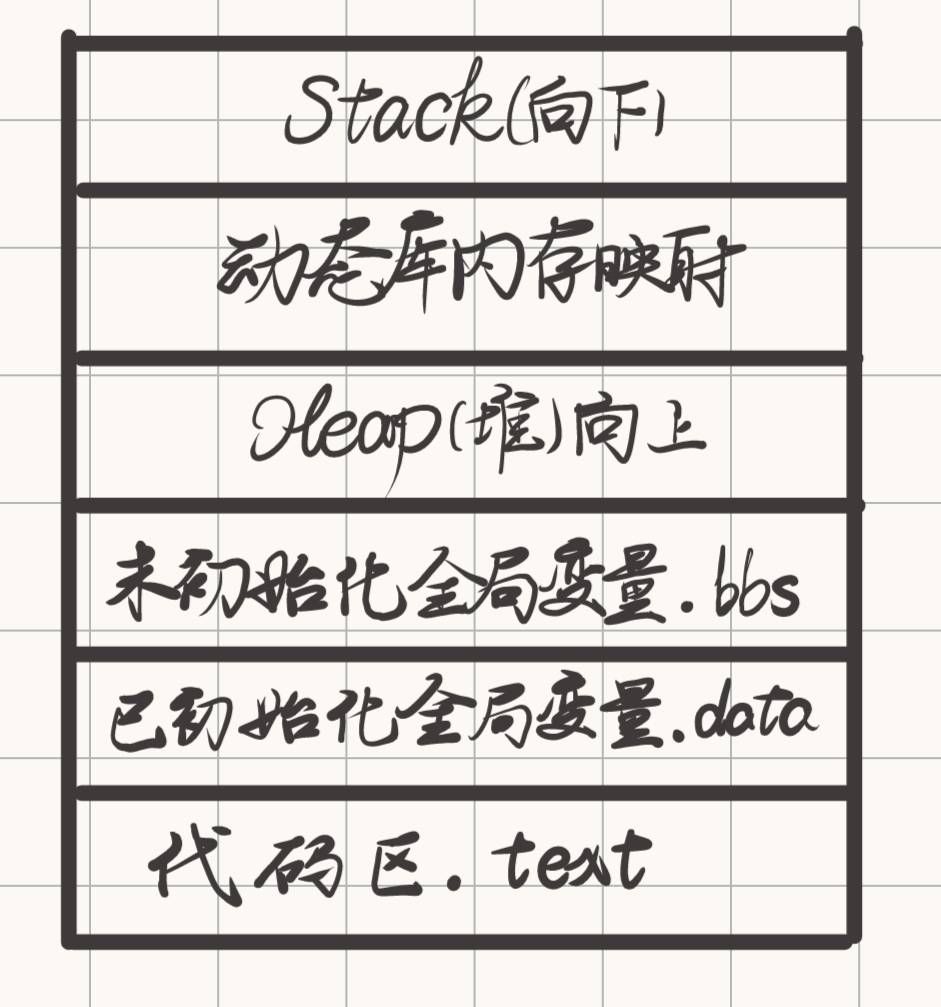
\includegraphics[width=0.42\textwidth]{Stack.jpg}
    \caption{堆栈分配} 
\end{figure}

查找空闲块的三个方法:
\begin{itemize}
    \item 1.首次适配:选择第一个合适的块。
    \item 2.下次适配:每次搜索从上次结束的地方开始。
    \item 3.最佳适配:选择大小合适的最小块。
\end{itemize}

\subsection{代码分析及填充}
对于速度($thru$)而言,我们需要关注$malloc$、$free$、$realloc$每次操作的复杂度。

对于内存利用率($util$)而言,我们需要关注$Internal \ Fragmentation$ (块内损失)和 $External \ Fragmentation$ (块是分散不连续的,无法整体利用)。

即我们$Free$和$Malloc$的时候要注意整体大块利用(例如合并$free$块、$realloc$的时候判断下一个块是否空闲)。

按照老师的要求,我首先选择实现双字对齐,隐式链表,采用首次适配。

按照$mm.c$中的内容补充一些宏定义以及函数定义,如下所示:

\begin{lstlisting}[language = C , title = { Define List } ]
    /* Basic constants and macros */

    #define WSIZE 4 // Word and header/footer size (bytes)
    #define DSIZE 8 // Double word size (bytes)
    #define CHUNKSIZE (1<<12) // Extend heap by this amount (bytes)

    #define MAX(x,y) ((x)>(y)?(x):(y)) // Maximum of two values

    #define PACK(size,alloc) ((size)|(alloc)) // Pack a size and allocated bit into a word

    #define GET(p)     (*(unsigned int *)(p)) // Read a word at address p
    #define PUT(p,val) (*(unsigned int *)(p) = (val)) // Write a word at address p
    #define GET_SIZE(p)  (GET(p) & ~0x7) // Read the size and allocated fields from address p
    #define GET_ALLOC(p) (GET(p) & 0x1) // Read the allocated field from address p

    // Given block ptr bp, compute address of its header and footer
    #define HDRP(bp) ((char *)(bp) - WSIZE)
    #define FTRP(bp) ((char *)(bp) + GET_SIZE(HDRP(bp)) - DSIZE)

    // Given block ptr bp, compute address of next and previous blocks
    #define NEXT_BLKP(bp) ((char *)(bp) + GET_SIZE(((char *)(bp) - WSIZE)))
    #define PREV_BLKP(bp) ((char *)(bp) - GET_SIZE(((char *)(bp) - DSIZE)))

\end{lstlisting}

接下来是需要定义的函数和辅助函数:

\begin{lstlisting}[language = C , title = { Function List } ]
    /* 内部编程的函数原型 */
    extern void *extend_heap(size_t words); // 扩展堆
    extern void *coalesce(void *bp); // 合并空闲块
    extern void *find_fit(size_t size); // 查找合适的空闲块
    extern void place(void *bp,size_t asize); // 分配空闲块
    extern int mm_init (void); // 初始化
    extern void *mm_malloc (size_t size); // 分配
    extern void mm_free (void *ptr); // 释放
    extern void *mm_realloc(void *ptr, size_t size); // 重新分配
    static char *heap_listp = 0; //指向块首的指针
\end{lstlisting}

接下来,我们对函数进行填充:

\begin{figure} [H]
    \centering
    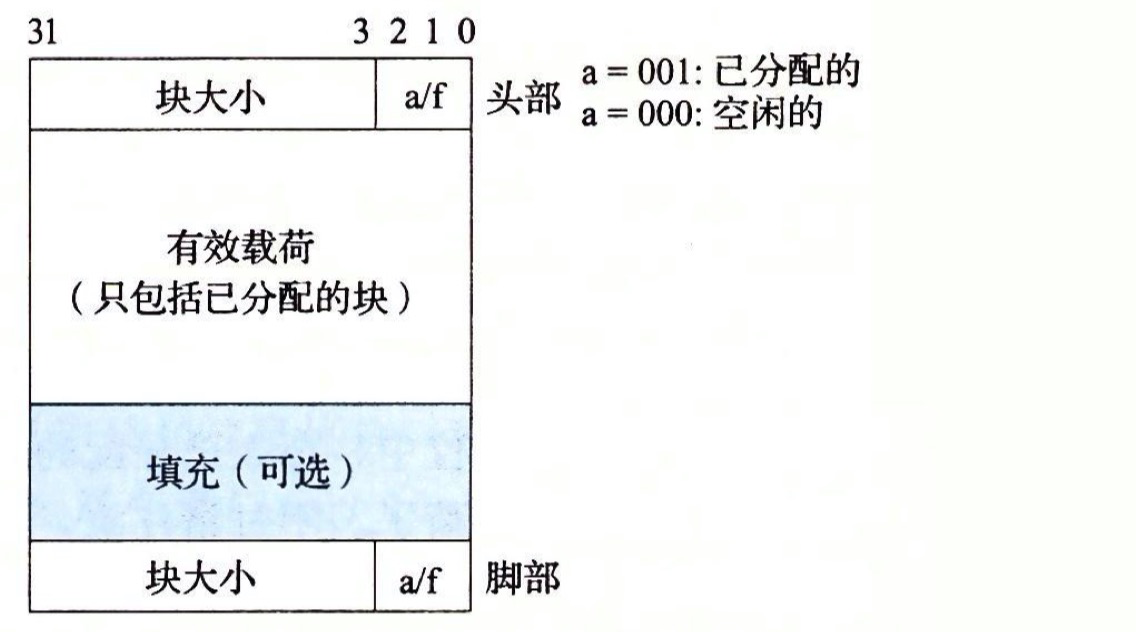
\includegraphics[width=0.42\textwidth]{BlockSize.png}
    \caption{块大小解释}
\end{figure}

\begin{lstlisting}[language = C , title = { mm\_init.c } ]
    int mm_init(void) 
    {
        /* Create the initial empty heap */
        if ((heap_listp = mem_sbrk(4*WSIZE)) == (void *)-1) // 申请4个字节
            return -1;
        PUT(heap_listp, 0);                          // Alignment padding
        PUT(heap_listp + (1*WSIZE), PACK(DSIZE, 1)); // Prologue header
        PUT(heap_listp + (2*WSIZE), PACK(DSIZE, 1)); // Prologue footer 
        PUT(heap_listp + (3*WSIZE), PACK(0, 1));     // Epilogue header
        heap_listp += (2*WSIZE);   // 指向序言块的头部                   
    
        /* Extend the empty heap with a free block of CHUNKSIZE bytes */
        if (extend_heap(CHUNKSIZE/WSIZE) == NULL)  // 扩展堆
            return -1; // 扩展失败
        return 0; // 成功
    }
\end{lstlisting}

\begin{itemize}
    \item 以堆底为起始位置,新建四个$WSIZE(4\ Bytes\ Or \ 32\ Bits)$大小的块
    \item 第一块什么都不放作为填充字
    \item 第二、三块分别作为序言块的头和脚
    \item 第四块作为结尾块
    \item 然后将指针后移两块,指向序言块脚部起始位置,随后调用$extend\_heap()$,申请$CHUNKSIZE$大小的空间,以备用。
\end{itemize}

\begin{lstlisting}[language = C , title = { Extend\_heap.c } ]
    static void *extend_heap(size_t words){
        char *bp; // 块指针
        size_t size; // 扩展大小
        size = (words%2) ? (words+1)*WSIZE : words*WSIZE;   // 8字节对齐
        if((long)(bp=mem_sbrk(size))==(void *)-1) 
            return NULL; // 申请失败
        PUT(HDRP(bp),PACK(size,0)); // 更新头部
        PUT(FTRP(bp),PACK(size,0)); // 更新尾部
        PUT(HDRP(NEXT_BLKP(bp)),PACK(0,1));     // 新结尾块 
        return coalesce(bp);     // 合并空闲块
    }
\end{lstlisting}

这个函数将堆扩容指定 $byte$ 大小。如果指定 $words$ 大小不为 $8$ 的倍数则向上取整使得每次扩容都是八字节对齐,
最后将头、脚内容补齐并将下一个块置为结尾块,最后调用$coalesce()$函数堆 $bp$ 进行合并操作后返回。

接下来,是$mm\_malloc()$函数:

此函数申请大小为 $size$ 的空间。$asize$ 为对 $size$ 进行$8$字节对齐检查后的大小,$extendsize$ 为取 $CHUNKSIZE$ 和 $asize$ 中较大的一个。

先用 $find\_fit()$ 在现有的块中进行搜索,如果搜索到了,即用 $place()$ 函数将 $asize$ 大小的空间放到$bp$中。
由于有可能全部分也可能分割成一个占用块和一个空闲块,所以不能粗暴的完全占用,要写一个 $place()$ 函数来分配。
如果找不到合适块,就向堆申请新空间,新空间的大小为$extendsize$,然后再用 $place()$ 函数放入。

\begin{lstlisting}[language = C , title = { mm\_malloc.c } ]
    void *mm_malloc(size_t size)
    {
        size_t asize; // 对齐大小
        size_t extendsize; // 扩展大小
        char *bp; // 块指针
        if(size ==0) return NULL; // 无效大小
        if(size <= DSIZE){
            asize = 2*(DSIZE); // 8字节对齐
        }else{
            asize = (DSIZE)*((size+(DSIZE)+(DSIZE-1)) / (DSIZE)); // 8字节对齐
        }
        if((bp = find_fit(asize))!= NULL){ // 查找合适的块
            place(bp,asize); // 分配
            return bp; // 返回块指针
        }
        extendsize = MAX(asize,CHUNKSIZE); // 申请大小
        if((bp = extend_heap(extendsize/WSIZE))==NULL){ // 扩展堆
            return NULL; // 申请失败
        }
        place(bp,asize); // 分配
        return bp; // 返回块指针
    }
\end{lstlisting}

接下来是$mm\_free()$函数:

此函数释放指针$ptr$所指向的块,将其标记为未分配状态,然后调用$coalesce()$函数合并空闲块。

\begin{lstlisting}[language = C , title = { mm\_free.c } ]
    void mm_free(void *bp)
    {
        if(bp == 0)
        return; // 无效指针
        size_t size = GET_SIZE(HDRP(bp)); // 获取块大小
        PUT(HDRP(bp),PACK(size,0)); // 标记为未分配
        PUT(FTRP(bp),PACK(size,0)); // 标记为未分配
        coalesce(bp); // 合并空闲块
    }
\end{lstlisting}

接下来是$mm\_realloc()$函数:

此函数重新分配指针$ptr$所指向的块,将其大小调整为$size$,如果$size$为$0$,则释放指针$ptr$所指向的块。

\begin{lstlisting}[language = C , title = { mm\_realloc.c } ]
    void *mm_realloc(void *ptr, size_t size) {
        size_t oldsize; // 旧块大小
        void *newptr; // 新块指针
        /* If size == 0 then this is just free, and we return NULL. */
        if(size == 0) { // 释放
        mm_free(ptr); // 释放
        return 0; // 返回NULL
        }
        /* If oldptr is NULL, then this is just malloc. */
        if(ptr == NULL) {
        return mm_malloc(size); // 申请
        }
        newptr = mm_malloc(size); // 申请
        /* If realloc() fails the original block is left untouched  */
        if(!newptr) {
        return 0;
        }
        /* Copy the old data. */
        oldsize = GET_SIZE(HDRP(ptr)); // 旧块大小
        if(size < oldsize) oldsize = size; // 复制旧数据
        memcpy(newptr, ptr, oldsize); // 复制
        /* Free the old block. */
        mm_free(ptr); // 释放
        return newptr; // 返回新块
    }
\end{lstlisting}

接下来是$place()$函数:

此函数将$asize$大小的块放入$bp$中,如果剩余空间大于$DSIZE$,则将剩余空间分割出来,否则将整个块分配出去。

\begin{lstlisting}[language = C , title = { place.c } ]
    static void place(void *bp,size_t asize){
        size_t csize = GET_SIZE(HDRP(bp)); // 当前块大小
        if((csize-asize)>=(2*DSIZE)){ // 剩余空间大于DSIZE
            PUT(HDRP(bp),PACK(asize,1)); // 更新头部
            PUT(FTRP(bp),PACK(asize,1)); // 更新尾部
            bp = NEXT_BLKP(bp); // 下一个块
            PUT(HDRP(bp),PACK(csize-asize,0)); // 更新头部
            PUT(FTRP(bp),PACK(csize-asize,0)); // 更新尾部
        }else{
            PUT(HDRP(bp),PACK(csize,1)); // 更新头部
            PUT(FTRP(bp),PACK(csize,1)); // 更新尾部
        }
    }
\end{lstlisting}

$coalesce()$函数:

此函数合并空闲块,如果前后块都是空闲块,则将其合并为一个块。

\begin{lstlisting} [language = C, title = calesec.c]
    static void *coalesce(void *bp){
    size_t  prev_alloc = GET_ALLOC(FTRP(PREV_BLKP(bp))); // 前块是否空闲
    size_t  next_alloc = GET_ALLOC(HDRP(NEXT_BLKP(bp))); // 后块是否空闲
    size_t size = GET_SIZE(HDRP(bp)); // 当前块大小
    if(prev_alloc && next_alloc) { // 前后块都忙碌
        return bp; // 返回当前块
    }else if(prev_alloc && !next_alloc){ // 前忙碌,后空闲
            size += GET_SIZE(HDRP(NEXT_BLKP(bp))); // 合并
            PUT(HDRP(bp), PACK(size,0)); // 更新头部
            PUT(FTRP(bp), PACK(size,0)); // 更新尾部
    }else if(!prev_alloc && next_alloc){ // 前空闲,后忙碌
        size += GET_SIZE(HDRP(PREV_BLKP(bp))); // 合并
        PUT(FTRP(bp),PACK(size,0)); // 更新尾部
        PUT(HDRP(PREV_BLKP(bp)),PACK(size,0)); // 更新头部
        bp = PREV_BLKP(bp); // 返回前块
    }else {
        size +=GET_SIZE(FTRP(NEXT_BLKP(bp)))+ GET_SIZE(HDRP(PREV_BLKP(bp))); // 前后都空闲
        PUT(FTRP(NEXT_BLKP(bp)),PACK(size,0)); // 更新尾部
        PUT(HDRP(PREV_BLKP(bp)),PACK(size,0)); // 更新头部
        bp = PREV_BLKP(bp); // 返回前块
    }
    return bp;
}
\end{lstlisting}

此函数将对传入的块指针进行前后检查,如果前面块或者后面块同样为空闲块,就进行合并。
首先获取前后块的空闲状态,然后进行条件判断,会出现四种情况:
\begin{itemize}
    \item 前后都忙碌
    \item 前忙碌,后空闲
    \item 前空闲,后忙碌
    \item 前后都空闲
\end{itemize}

$find\_fit()$函数:

此函数在空闲块中查找合适的块,如果找到了就返回块指针,否则返回$NULL$。

\begin{lstlisting} [language = C, title = find\_fit.c]
    static void *find_fit(size_t asize){
        void *bp; // 遍历指针
        for(bp = heap_listp; GET_SIZE(HDRP(bp))>0; bp = NEXT_BLKP(bp)){ // 从堆底开始遍历
            if(!GET_ALLOC(HDRP(bp)) && (asize <= GET_SIZE(HDRP(bp)))){ // 找到合适的块
                return bp; // 返回块指针
            }
        }
        return NULL;
    }
\end{lstlisting}

这个函数从堆底开始遍历,如果找到了一个空闲块且大小大于等于$asize$,就返回这个块的指针,否则返回$NULL$。

\subsection{实验结果}
将补充好的$mm.c$文件导入Linux系统,使用$make$命令编译,然后使用$mdriver$工具进行测试,得到如下结果:
\begin{itemize}
    \item make clean
    \item make
    \item ./mdriver -av -t traces/
\end{itemize}

\begin{figure} [H]
    \centering
    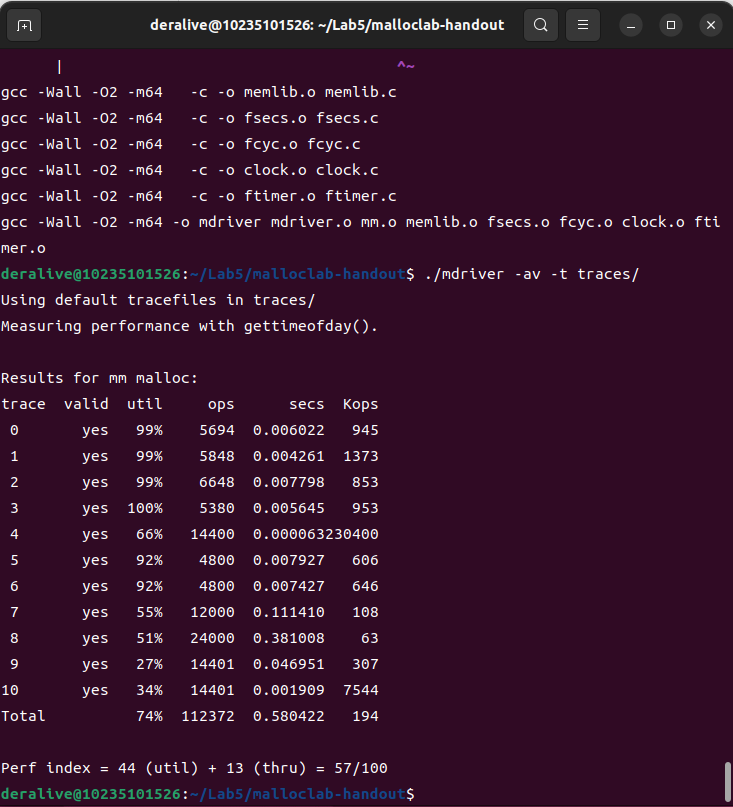
\includegraphics[width=0.5\textwidth]{Result.png}
    \caption{Result}
\end{figure}

可以看到,我们获得了$44$的$Util$分,$13$的$Thru$分,总分为$57$。

这个分数是一个看起来尚未及格的分数,我后续将考虑使用其他方法来优化。
